%\documentclass[tikz,border=5pt]{standalone}
\documentclass{article}
\usepackage{graphicx}

\usepackage{tikz}
\usepackage{amsmath, amssymb, bm}
\usepackage{xcolor}
\usetikzlibrary{
	positioning,
	arrows.meta,
	decorations.pathmorphing,
	decorations.pathreplacing,
	calc
}

% 自定义颜色
\definecolor{mymauve}{RGB}{160,90,180}
\definecolor{mygreen}{RGB}{60,150,90}


\begin{document}
	


\begin{figure}
	\begin{tikzpicture}
		\node[circle, draw, thick] (n1) {};
		\node[circle, draw, thick, right=1em of n1] (n2) {};
		\node[circle, draw, thick, right=1em of n2] (n3) {};
		\node[circle, draw, thick, right=1em of n3] (n4) {};
		\node[circle, draw, thick, right=1em of n4] (n5) {};
		\node[circle, draw, thick, right=1em of n5] (n6) {};
		\node[circle, draw, thick, right=1em of n6] (n7) {};
		\node[circle, draw, thick, right=1em of n7] (n8) {};
		\path (n4) -- (n5) node[circle, draw, thick, pos=.5,above=5em] (B) {\begin{tikzpicture}
				\draw[thick] (0,-0.1) -- (0.25, 0);
				\draw[thick] (0.245,-0.002) -- (0.445, 0.248);
		\end{tikzpicture}};
		\node[draw, thick, circle, above=5em of B] (O) {$\alpha_{ij}$};
		
		\foreach \x in {1,...,7}
		\draw[-stealth, thick] (n\x) -- (B);
		
		\draw[-stealth, thick] (n8) -- node[right, xshift=0.5em] {$\vec{\bf a}$} (B);
		
		\draw[-stealth, thick] (B) -- node[sloped, pos=0.5, yshift=-0.7em] {softmax$_j$} (O);
		
		\draw [very thick, decoration={brace,mirror,amplitude=7},decorate] ([yshift=-2mm]n1.west) --node[below=3mm]{${\bf W}\vec{h}_i$} ([yshift=-2mm]n4.east);
		\draw [very thick, decoration={brace,mirror,amplitude=7},decorate] ([yshift=-2mm]n5.west) --node[below=3mm]{${\bf W}\vec{h}_j$} ([yshift=-2mm]n8.east);
	\end{tikzpicture}\hfill 
	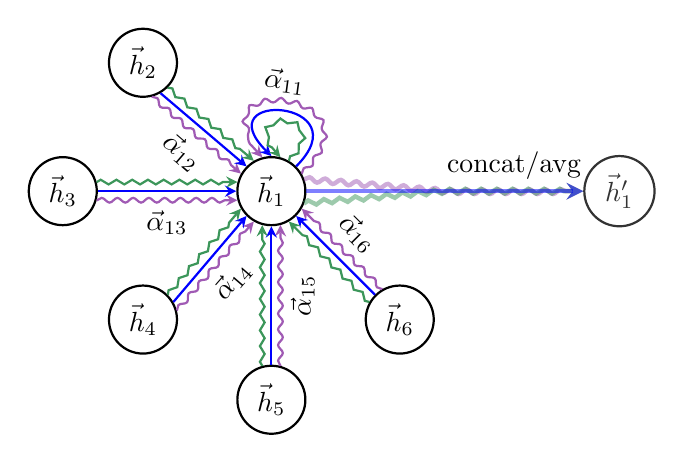
\begin{tikzpicture}
		\node[circle, draw, thick] (h1) {$\vec{h}_1$};
		%\node[circle, draw, thick, above right=of h1] (h2) {$\vec{h}_2$};
		%\node[circle, draw, thick, above=5em of h1] (h3) {$\vec{h}_3$};
		\node[circle, draw, thick, above left=of h1] (h4) {$\vec{h}_2$};
		\node[circle, draw, thick, left=5em of h1] (h5) {$\vec{h}_3$};
		\node[circle, draw, thick, below left=of h1] (h6) {$\vec{h}_4$};
		\node[circle, draw, thick, below=5em of h1] (h7) {$\vec{h}_5$};
		\node[circle, draw, thick, below right=of h1] (h8) {$\vec{h}_6$};
		
		\draw[-stealth, mymauve, thick,decoration={snake, pre length=0.01mm, segment length=2mm, amplitude=0.3mm, post length=1.5mm}, decorate] (h8.120) -- node[sloped, above, black] {$\vec{\alpha}_{16}$} (h1.-30);
		\draw[-stealth, blue, thick] (h8.135) -- (h1.-45);
		\draw[-stealth, mygreen, thick, decoration={zigzag, pre length=0.01mm, segment length=2mm, amplitude=0.3mm, post length=1.5mm}, decorate] (h8.150) -- (h1.-60);
		
		%\draw[-stealth, mymauve, thick,decoration={snake, pre length=0.01mm, segment length=2mm, amplitude=0.3mm, post length=1.5mm}, decorate] (h2.210) -- node[sloped, above, black] {$\vec{\alpha}_{12}$} (h1.60);
		%\draw[-stealth, blue, thick] (h2.225) -- (h1.45);
		%\draw[-stealth, mygreen, thick, decoration={zigzag, pre length=0.01mm, segment length=2mm, amplitude=0.3mm, post length=1.5mm}, decorate] (h2.240) -- (h1.30);
		
		
		%\draw[-stealth, mymauve, thick,decoration={snake, pre length=0.01mm, segment length=2mm, amplitude=0.3mm, post length=1.5mm}, decorate] (h3.255) -- node[sloped, below, black] {$\vec{\alpha}_{13}$}(h1.105);
		%\draw[-stealth, blue, thick] (h3.270) -- (h1.90);
		%\draw[-stealth, mygreen, thick, decoration={zigzag, pre length=0.01mm, segment length=2mm, amplitude=0.3mm, post length=1.5mm}, decorate] (h3.285) -- (h1.75);
		
		\draw[-stealth, mymauve, thick,decoration={snake, pre length=0.01mm, segment length=2mm, amplitude=0.3mm, post length=1.5mm}, decorate] (h1.30) to[looseness=7] node[sloped, above, black] {$\vec{\alpha}_{11}$}(h1.105);
		\draw[-stealth, blue, thick] (h1.45) to[looseness=9] (h1.90);
		\draw[-stealth, mygreen, thick, decoration={zigzag, pre length=0.01mm, segment length=2mm, amplitude=0.3mm, post length=1.5mm}, decorate] (h1.60) to[looseness=20] (h1.75);
		
		
		
		\draw[-stealth, mymauve, thick,decoration={snake, pre length=0.01mm, segment length=2mm, amplitude=0.3mm, post length=1.5mm}, decorate] (h4.285) -- node[sloped, below, black] {$\vec{\alpha}_{12}$}(h1.150);
		\draw[-stealth, blue, thick] (h4.300) -- (h1.135);
		\draw[-stealth, mygreen, thick, decoration={zigzag, pre length=0.01mm, segment length=2mm, amplitude=0.3mm, post length=1.5mm}, decorate] (h4.315) -- (h1.120);
		
		\draw[-stealth, mymauve, thick,decoration={snake, pre length=0.01mm, segment length=2mm, amplitude=0.3mm, post length=1.5mm}, decorate] (h5.-15) -- node[sloped, below, black] {$\vec{\alpha}_{13}$}(h1.195);
		\draw[-stealth, blue, thick] (h5.0) -- (h1.180);
		\draw[-stealth, mygreen, thick, decoration={zigzag, pre length=0.01mm, segment length=2mm, amplitude=0.3mm, post length=1.5mm}, decorate] (h5.15) -- (h1.165);
		
		\draw[-stealth, mymauve, thick,decoration={snake, pre length=0.01mm, segment length=2mm, amplitude=0.3mm, post length=1.5mm}, decorate] (h6.15) -- node[sloped, below, black] {$\vec{\alpha}_{14}$}(h1.240);
		\draw[-stealth, blue, thick] (h6.30) -- (h1.225);
		\draw[-stealth, mygreen, thick, decoration={zigzag, pre length=0.01mm, segment length=2mm, amplitude=0.3mm, post length=1.5mm}, decorate] (h6.45) -- (h1.210);
		
		\draw[-stealth, mymauve, thick,decoration={snake, pre length=0.01mm, segment length=2mm, amplitude=0.3mm, post length=1.5mm}, decorate] (h7.75) -- node[sloped, below, black] {$\vec{\alpha}_{15}$}(h1.-75);
		\draw[-stealth, blue, thick] (h7.90) -- (h1.-90);
		\draw[-stealth, mygreen, thick, decoration={zigzag, pre length=0.01mm, segment length=2mm, amplitude=0.3mm, post length=1.5mm}, decorate] (h7.105) -- (h1.-105);
		
		\node[circle, draw, thick, right=10em of h1, opacity=0.8] (hp) {$\vec{h}_1'$};
		
		\coordinate[right=5em of h1] (A);
		
		\draw[-stealth,  mymauve, opacity=0.5, ultra thick,decoration={snake, pre length=0.01mm, segment length=2mm, amplitude=0.3mm, post length=1.5mm}, decorate] (h1.20) -- (A) -- (hp);
		\draw[-stealth, mygreen, opacity=0.5, ultra thick,decoration={zigzag, pre length=0.01mm, segment length=2mm, amplitude=0.3mm, post length=1.5mm}, decorate] (h1.-20) -- (A) -- (hp);
		\draw[-stealth, blue, opacity=0.5, ultra thick] (h1.0) -- (A) -- node[black, above, opacity=1.0] {concat/avg} (hp);
	\end{tikzpicture}
%	\caption{{\bf Left:} The attention mechanism $a({\bf W}\vec{h}_i, {\bf W}\vec{h}_j)$ employed by our model, parametrized by a weight vector $\vec{\bf a} \in \mathbb{R}^{2F'}$, applying a LeakyReLU activation. {\bf Right:} An illustration of multi-head attention (with $K=3$ heads) by node 1 on its neighborhood. Different arrow styles and colors denote independent attention computations. The aggregated features from each head are concatenated or averaged to obtain $\vec{h}_1'$.}
	\label{figattn}
\end{figure}

\end{document}
